% Chương 2

\chapter{THIẾT KẾ HỆ THỐNG} % Tên của chương

\label{Chapter2} % Để trích dẫn chương này ở chỗ nào đó trong bài, hãy sử dụng lệnh \ref{Chapter2} 

%----------------------------------------------------------------------------------------

% Định nghĩa một số lệnh cần thiết để điều chỉnh định dạng cho một số nội dung nhất định trong bài

%\newcommand{\keyword}[1]{\textbf{#1}}
%\newcommand{\tabhead}[1]{\textbf{#1}}
%\newcommand{\code}[1]{\texttt{#1}}
%\newcommand{\file}[1]{\texttt{\bfseries#1}}
%\newcommand{\option}[1]{\texttt{\itshape#1}}

%----------------------------------------------------------------------------------------

\section{Giới thiệu}
Dựa vào lý thuyết của thuật toán điều khiển PID, tiểu luận này đã xây dựng mô hình thực tế có sử dụng bộ điều khiển này đó là mô hình điều khiển vị trí góc quay động cơ DC Encoder.


\section{Điều khiển vị trí góc quay động cơ DC Encoder sử dụng thuật toán PID}

\subsection{Tổng quan}
Bằng việc sử dụng thuật toán điều khiển PID, có thể điều khiển vị trí của động cơ DC Encoder dựa vào đĩa Encoder được gắn sẵn trên trục động cơ. 

\subsection{Lý thuyết}

Sử dụng động cơ DC giảm tốc GA25 Encoder. Động cơ có gắn thêm phần Encoder là một đĩa Encoder 11 xung, hai kênh A và B để có thể trả xung về vi điều khiển. Dựa vào giá trị xung trả về, có thể biết được vị trí hiện tại của đĩa. Từ đó có thể dễ dàng xác định vị trí hoặc vận tốc của động cơ. Cùng với việc sử dụng thuật toán điều khiển PID, vị trí hay tốc độ của động cơ được điều khiển một cách chính xác. 

\begin{figure}[h!]
	\centering
	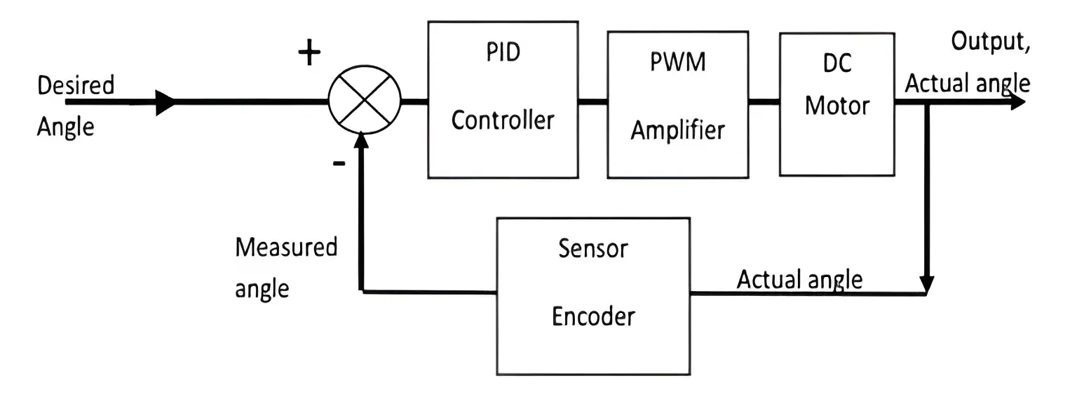
\includegraphics[width=0.8\textwidth]{pid_sd.png}
	\caption[Sơ đồ khối hệ thống]{Sơ đồ khối hệ thống}
	\label{fig:Sơ đồ khối hệ thống}
\end{figure}


\subsection{Một số chức năng được sử dụng trong mô hình}
\subsubsection{Ngắt ngoài - External Interrupt}

Ngắt (interrupt) là những lời gọi hàm tự động khi hệ thống sinh ra một sự kiện. Những sự kiện này được nhà sản xuất vi điều khiển thiết lập bằng phần cứng và được cấu hình trong phần mềm bằng những tên gọi cố định. Ngắt giúp chương trình gọn nhẹ và xử lý nhanh hơn. Ví dụ với việc kiểm tra một nút nhấn có được nhấn hay không, việc kiểm tra trạng thái nút nhấn trong vòng lặp while(1) của chương trình có thể gây ảnh hưởng tới chương trình chính. Với việc sử dụng ngắt, chỉ cần nối nút nhấn đến đúng chân có hỗ trợ ngắt, sau đó cài đặt ngắt sẽ sinh ra khi trạng thái nút chuyển từ HIGH->LOW. Thêm một tên hàm sẽ gọi khi ngắt sinh ra. Như vậy đoạn chương trình ngắt sẽ cho biết trạng thái nút nhấn.

Có bốn trạng thái của ngắt bao gồm:

\begin{itemize}
	
	\item LOW: kích hoạt liên tục khi trạng thái chân digital có mức thấp
	\item HIGH: kích hoạt liên tục khi trạng thái chân digital có mức cao.
	\item RISING: kích hoạt khi trạng thái của chân digital chuyển từ mức điện áp thấp sang mức điện áp cao.
	\item FALLING: kích hoạt khi trạng thái của chân digital chuyển từ mức điện áp cao sang mức điện áp thấp.
	
\end{itemize}

Trong mô hình này việc xác định chiều quay của động cơ sẽ được thực hiện bằng cách sử dụng ngắt INT0 (chân PD2) ở chế độ RISING, kênh A của Encoder được nối với chân PD2, kênh B được nối vào chân PD3. Như vậy mỗi khi ngắt được tạo ra, bằng cách đọc giá trị ở kênh B, có thể xác định được chiều quay của động cơ.

\begin{figure}[h!]
	\centering
	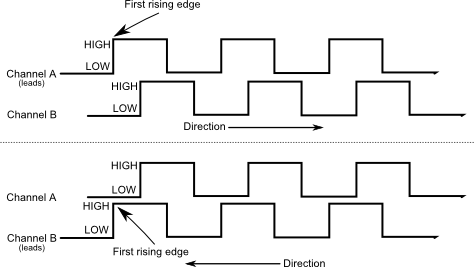
\includegraphics[width=0.8\textwidth]{encoder.png}
	\caption[Xác định chiều quay của động cơ DC Encoder]{Xác định chiều quay của động cơ DC Encoder}
	\label{fig:Xác định chiều quay của động cơ DC Encoder}
\end{figure}
\newpage
\subsubsection{Tạo xung Fast PWM}

\begin{figure}[h!]
	\centering
	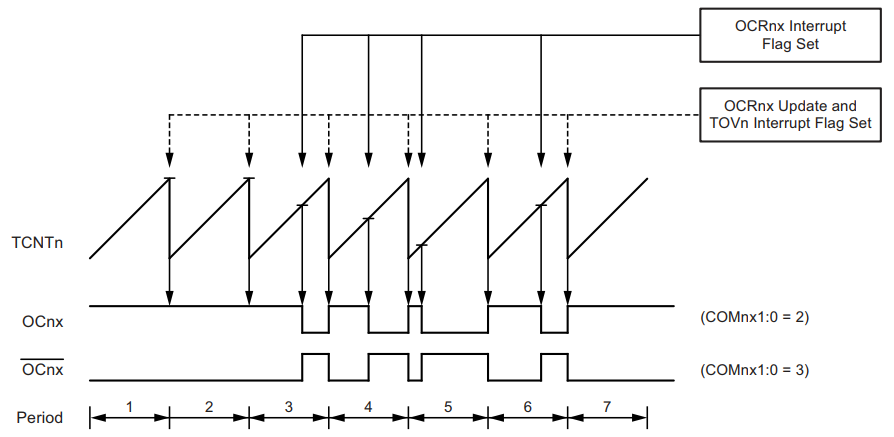
\includegraphics[width=0.8\textwidth]{pwm.png}
	\caption[Tạo xung Fast PWM]{Tạo xung Fast PWM}
	\label{fig:Tạo xung Fast PWM}
\end{figure}

WGM2:0 = 0b011 hoặc 0b111.

Counter chạy từ 0x00 tới TOP rồi được reset lại về 0x00. 

TOP = MAX khi WGM2:0 = 0b011; TOP = OCRxA nếu WGM2:0 = 0b111 

Khi CTNTx = OCRxn, tạo ra phản ứng tại chân OCxn. Phản ứng tại chân OCxn tùy thuộc vào giá trị của bit COMxn1:0
\newpage
Ngắt được tạo ra (nếu cho phép) khi CTNTx  = TOP.

\begin{figure}[h!]
	\centering
	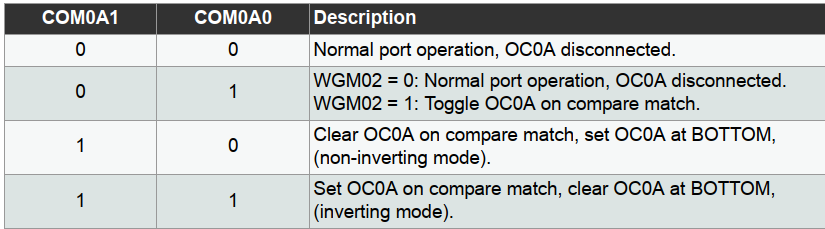
\includegraphics[width=0.8\textwidth]{pwm2.png}
	\caption[Chế độ trong tạo xung Fast PWM]{Chế độ tạo xung Fast PWM}
	\label{fig:Chế độ tạo xung Fast PWM}
\end{figure}

Tần số PWM tại đầu ra OCxn chỉ phụ thuộc vào tần số clock đưa vào Timer.

Giá trị trên thanh ghi so sánh OCRxn quyết định mức năng lượng được kích hoạt trong mỗi chu kì. 

Công thức tính chu kì xung PWM: 

\begin{align}
	f_{OCxA} = \frac{f_{IO}}{2.d.MAX}
\end{align}

Trong đó:
\begin{itemize}
	
	\item d : hệ số chia clock của timer
	\item $f_{IO}$ : Tần số clock của IO
	\item $f_{OCxA}$ : Tần số xung tại đầu ra so sánh OCxA
	
\end{itemize}
\newpage
Như vậy, bằng việc tạo xung Fast PWM, có thể dễ dàng điều khiển tốc độ quay của động cơ thông qua module L298N.

\begin{figure}[h!]
	\centering
	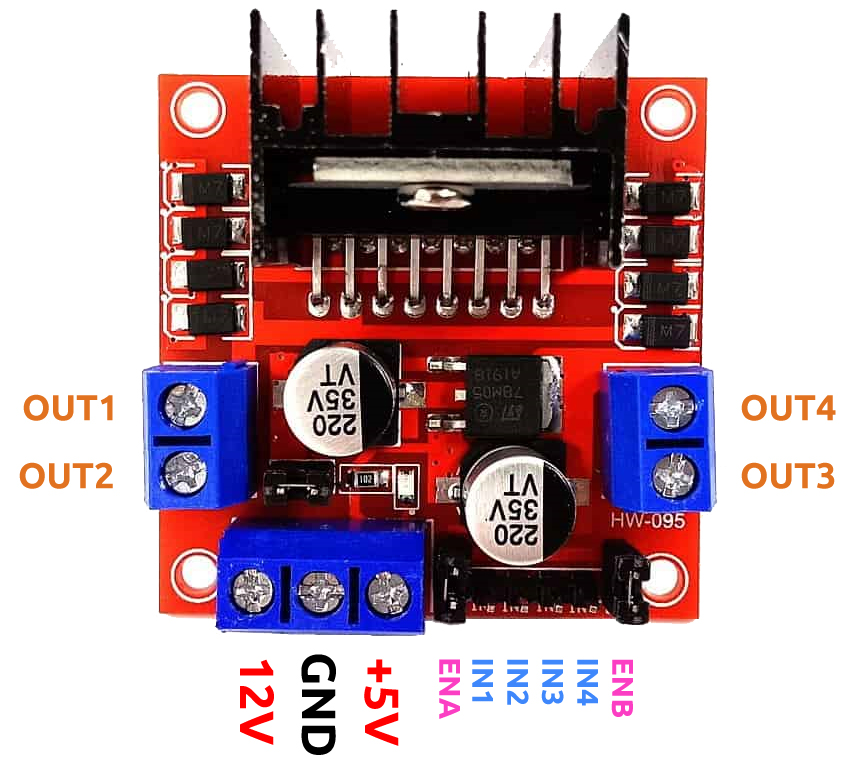
\includegraphics[width=0.6\textwidth]{l298n.jpg}
	\caption[Module L298N]{Module L298N}
	\label{fig:Module L298N}
\end{figure}

Chiều quay của động cơ được thay đổi bằng việc thay đổi giá trị trên chân PD6 nối với IN3 của module và PD7 nối với INT4 của module.
\newpage

\subsubsection{Analog to Digital Converter (ADC)}

Sơ đồ khối ADC

\begin{figure}[h!]
	\centering
	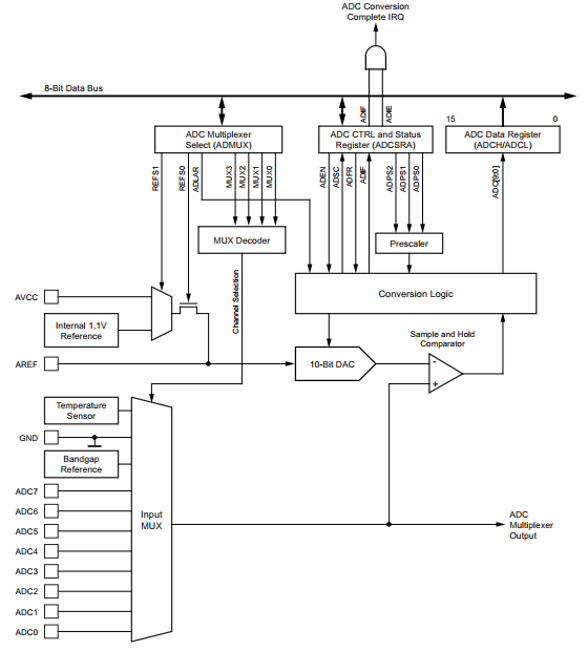
\includegraphics[width=0.8\textwidth]{ADC_sd.png}
	\caption[Sơ đồ khối ADC trên ATmega328p]{Sơ đồ khối ADC trên ATmega328p}
	\label{fig:Sơ đồ khối ADC trên ATmega328p}
\end{figure}

\begin{figure}[h!]
	\centering
	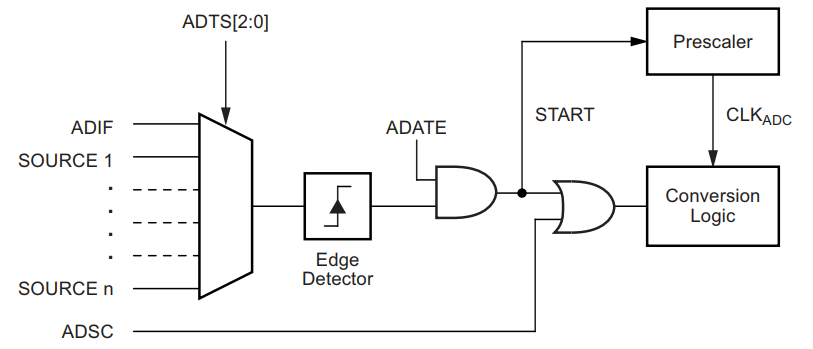
\includegraphics[width=0.8\textwidth]{ADC_hd.png}
	\caption[Hoạt động của khối ADC]{Hoạt động của khối ADC}
	\label{fig:Hoạt động của khối ADC}
\end{figure}

ADTS (ADC Trigger Select): Chọn nguồn đầu vào cho bộ ADC

ADSC (ADC Start Conversion): Bắt đầu chuyển đổi

SOURCE: Nguồn đầu vào analog, ADC0 đến ADC5, tương ứng với PC0 đến PC5

ADATE (ADC Auto Trigger Enable): Tự động chuyển đổi

ADC cần clock trong tầm 50kH tới 200 kHz để đảm bảo độ phân giải tối đa 10 bit.
Trong trường hợp không yêu cầu độ phân giải cao, cần tăng tốc độ lấy mẫu, ADC clock có thể được cấu hình cao hơn 200 kHz.

Việc thay đổi tốc độ ADC clock dựa trên các bit ADPS[2:0] trên thanh ghi ADCSRA.

Thời gian cho 1 lần chuyển đổi thường là 13 ADC clock. Ngoại trừ lần chuyển đổi đầu tiên cần 25 ADC clock.
 
Một số thanh ghi quản lý ADC:
 
\begin{itemize}
	
	\item Thanh ghi ADMUX (ADC multiplexer Selection)
	Là thanh ghi lựa chọn điện áp tham chiếu, căn lề thanh ghi kết quả và lựa chọn kênh đầu vào cho ADC.
	
	\item Thanh ghi ADCSRA (ADC Control and Status Register A)
	Cấu hình và lựa chọn tốc độ lấy mẫu.
	
	\item Thanh ghi ADCSRB (ADC Control and Status Register B)
	Lựa chọn nguồn kích hoạt chế độ lấy mẫu tự động (Auto Conversion).
	
	\item Thanh ghi DIDR0 (Digital Input Disable)
	Loại bỏ đầu vào số cho các Input.
	
	\item Thanh ghi ADCL và ADCH (ADC Data Register)
	Thanh ghi chứa kết quả của quá trình chuyển đổi.
	
\end{itemize}

Giá trị của ADC nằm trong khoảng từ 0 - 1023 sau đó được chuyển về từ 0 - 360 ứng với 360 độ của động cơ. Giá trị ADC này sau đó được chuyển đổi tiếp thành giá trị của đĩa encoder tương ứng với góc quay của động cơ.

\subsubsection{Giao tiếp TWI}

Nhằm thuận tiện cho quá trình theo dõi hoạt động của hệ thống, mô hình sử dụng màn hình LCD1602 được gắn module I2C PCF8574, giao tiếp TWI với vi điều khiển. Các thống số như SP, PV hay giá trị góc quay sẽ được hiển thị lên LCD.

Chuẩn giao tiếp TWI được nghiên cứu và phát triển bởi Atmel, thực chất chính là chuẩn I2C của Philips Semiconductor với cái tên khác. Đây là giao tiếp sử dụng 2 dây kết nối là SCK (Serial Clock) và SDA (Serial Data), là chuẩn giao tiếp không đồng bộ và bán song công (half-duplex). Hai dây SCK và SDA cần điện trở kéo lên (Pull up resistor). Chế độ làm việc theo mô hình Multi-Master với cơ chế phân xử xung đột thiết bị chủ. Tốc độ clock cao nhất đạt 400 kHz. Slave được định địa chỉ 7 bit bằng lập trình, hỗ trợ General Call.

Các chế độ là việc của giao tiếp TWI:
\begin{itemize}
	
	\item Master: Là thiết bị khởi tạo và kết thúc giao tiếp. Master sẽ tạo ra xung clock trên đường SCL. Master sẽ gửi địa chỉ yêu cầu kết nối với slave trên bus.
	\item Slave: Thiết bị được master gửi địa chỉ yêu cầu kết nối trên bus.
	\item Transmitter (Bộ truyền): Là thiết bị gửi dữ liệu lên trên bus.
	\item Receiver (Bộ nhận): Là thiết bị đọc dữ liệu trên bus.
	\item Như vậy sẽ có 4 chế độ cho thiết bị TWI là Master-transmit, Master-receive, Slave-transmit và Slave-receive.

\end{itemize}



\subsubsection{Giao tiếp USART}
USART (Universal Synchronous and Asynchronous serial Receiver and Transmitter): Là bộ truyền nhận thông tin nối tiếp, dữ liệu được truyền theo từng bit liên tục với nhau.

Có 2 chế độ: Đồng bộ và không đồng bộ

\begin{itemize}
	
	\item Master: Không đồng bộ: Hai bên thu và nhận có nguồn clock riêng, dữ liệu được gửi theo từng byte (thêm bit start, stop và parity). Thường dung trong truyền dữ liệu giữa các thiết bị khác nhau.
	\item Slave: Đồng bộ: Hai bên thu và nhận sử dụng chung 1 nguồn clock, dữ liệu được gửi liên tục không cần bit start, stop và parity. Thường dung trong truyền dữ liệu on board.
	
\end{itemize}

Giao thức hoạt động ở chế độ song công (Full duplex), hỗ trợ khung truyền tin 5,6,7,8 hoặc 9 bit dữ liệu, 1 hoặc 2 bit dừng (stop bit), hỗ trợ kiểm tra lỗi (Check parity). Có 3 ngắt: Ngắt TX, ngắt TX data Register empty và ngắt RX.

Sơ đồ khối USART:

\begin{figure}[h!]
	\centering
	\includegraphics[width=0.8\textwidth]{USART.png}
	\caption[Sơ đồ khối USART]{Sơ đồ khối USART}
	\label{fig:Sơ đồ khối USART}
\end{figure}

Chia làm 3 khối chính: Clock Generator, Transmitter và Receiver.

Chân XCK (PD4) chỉ dung trong chế độ đồng bộ.

Chân TX (PD1) là chân truyền tín hiệu (Transmit).

Chân RX (PD0) là chân nhận tín hiệu (Receiver).

Giao tiếp USART được sử dụng nhằm phục vụ xử lý số liệu và vẽ đồ thị hoạt động của hệ thống.


\subsection{Ảnh mô hình}

Vỏ hộp và các linh kiện được thiết kế và in 3D. Mô hình điều khiển vị trí góc động cơ. Có thể thay đổi giá trị SP bằng cách vặn chiết áp. Giá trị SP sau đó được hiển thị lên màn hình LCD1602, đồng thời động cơ cũng quay một góc có độ lớn đúng bằng độ lớn của giá trị SP. Mỗi vạch trên đĩa ứng với 10 độ, mũi trên trên trục động cơ sẽ giúp xác định góc quay của động cơ. 

\begin{figure}[h!]
	\centering
	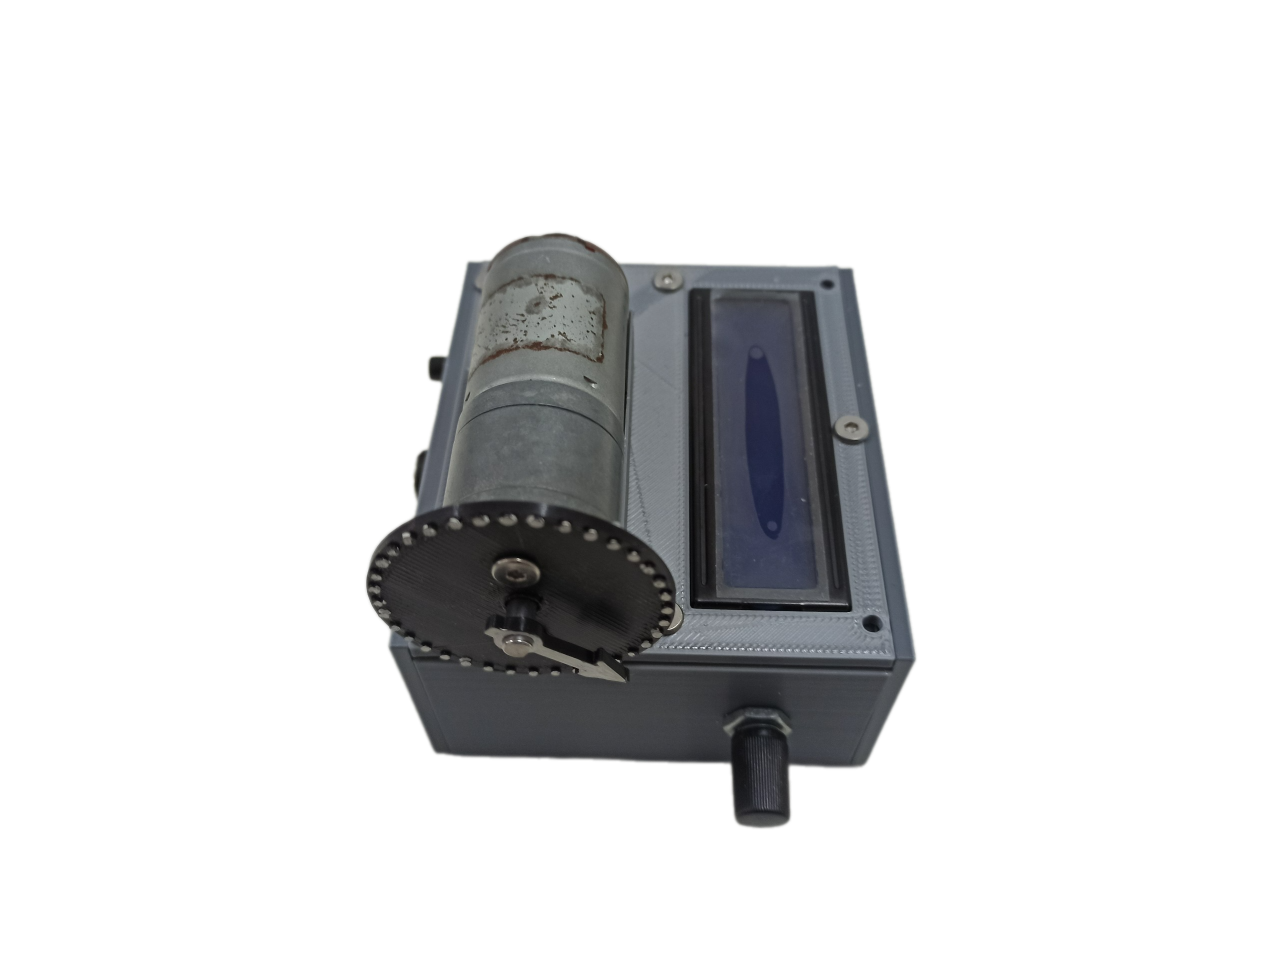
\includegraphics[width=0.8\textwidth]{dc_enc.jpg}
	\caption[Mô mình điều khiển vị trí góc quay động cơ]{Mô mình điều khiển vị trí góc quay động cơ}
	\label{fig:Mô mình điều khiển vị trí góc quay động cơ}
\end{figure}
\newpage
\subsection{Sơ đồ linh kiện}

Mô hình được sử dụng một nguồn 12V cung cấp nguồn nuôi cho động cơ, hai chân ENA và ENB của L298N cần được nối với chân xung của vi điều khiển, chân GND cần được nối chung cho toàn mạch. Chi tiết sơ đồ chân nối được ghi ở phần phụ lục \ref{AppendixB}

\begin{figure}[h!]
	\centering
	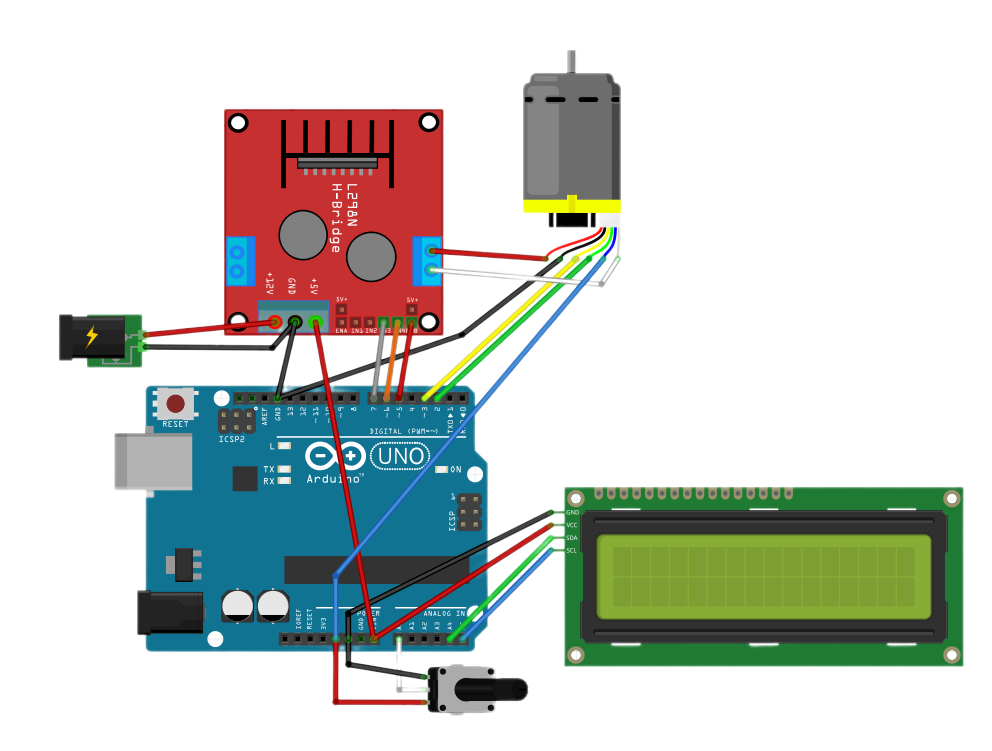
\includegraphics[width=0.8\textwidth]{sche_dc-enc.png}
	\caption[Sơ đồ chân mô mình điều khiển vị trí góc quay động cơ]{Sơ đồ chân mô mình điều khiển vị trí góc quay động cơ}
	\label{fig:Sơ đồ chân mô mình điều khiển vị trí góc quay động cơ}
\end{figure}
\newpage
\subsection{Thiết kế mạch in}

Mạch in của mô hình được thiết kế bằng phần mềm Altium.

\begin{figure}[h!]
	\centering
	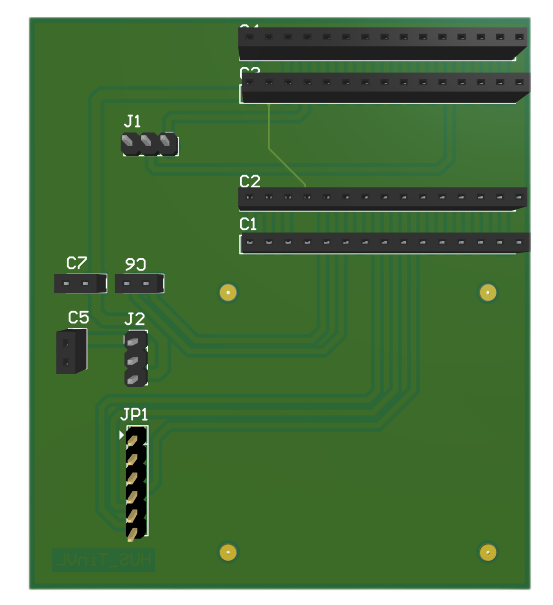
\includegraphics[width=0.8\textwidth]{pcb_dc-enco.png}
	\caption[Thiết kế mạch in mô mình điều khiển vị trí góc quay động cơ DC Encoder]{Thiết kế mạch in mô mình điều khiển vị trí góc quay động cơ DC Encoder}
	\label{fig:Thiết kế mạch in mô mình điều khiển vị trí góc quay động cơ DC Encoder}
\end{figure}
\newpage
\subsection{Thiết kế vỏ hộp}
 Vỏ hộp của mô hình được thiết kế bằng phần mềm Fusion360 sau đó được in 3D.
 
 \begin{figure}[h!]
 	\centering
 	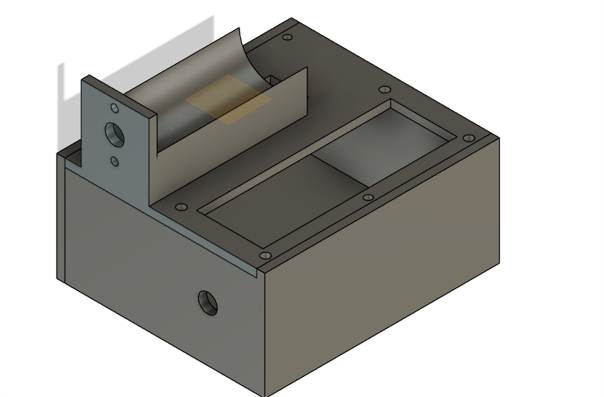
\includegraphics[width=0.8\textwidth]{hop.png}
 	\caption[Vỏ hộp của mô hình được vẽ 3D]{Vỏ hộp của mô hình được vẽ 3D}
 	\label{fig:Vỏ hộp của mô hình được vẽ 3D}
 \end{figure}


\subsection{Phương pháp tìm $K_p$, $K_i$, $K_d$}
\subsubsection{Với bộ điều khiển PID}
Sử dụng phương pháp Ziegler-Nichols 2 để tìm độ lợi cho hệ thống, cùng với đó là hiệu chỉnh thủ công và tiến hành khảo sát để tìm ra ba hằng số độ lợi cho mô hình. Ở mô hình này, ba hằng số độ lợi $K_p$, $K_i$  và $K_d$ lần lượt là 6,75 ; 12,14 và 0,22.

\subsubsection{Với bộ điều khiển PD}
Bằng cách lược bỏ khâu tích phân trong bộ điều khiển PID, bộ điều khiển PD được xây dựng cho mô hình điều khiển vị trí động cơ DC Encoder. Tiến hành tìm thông số $K_p$, $K_d$ cho hệ thống. Ở đây, hai giá trị $K_p$ và $K_d$ lần lượt được xác định bằng 6,7 và 0,2.
\newpage
\subsection{Kết quả}
Hệ thống hoạt động ổn định với các giá trị góc được đặt ra. Khi ta thay đổi setpoint bằng cách vặn chiết áp, giá trị này sẽ được hiển thị lên màn hình LCD, đồng thời động cơ cũng quay một góc bằng giá trị setpoint. Cụ thể trong từng bộ điều khiển PD và PID sẽ cho các kết quả như sau.

\subsubsection{Với bộ điều khiển PD}

Khảo sát hoạt động của hệ thống với bộ điều khiển PD cho thấy hệ thống hoạt động tương đối chính xác, phản hồi nhanh. 

 \begin{figure}[h!]
	\centering
	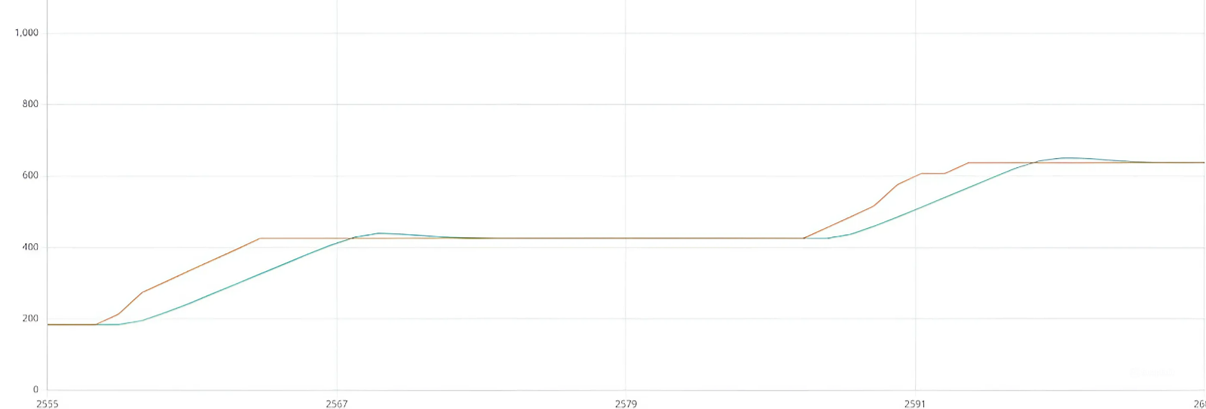
\includegraphics[width=0.9\textwidth]{pd1.png}
	\caption[Hoạt động của hệ thống với bộ điều khiển PD (1)]{Hoạt động của hệ thống với bộ điều khiển PD (1)}
	\label{fig:Hoạt động của hệ thống với bộ điều khiển PD (1)}
\end{figure}

Tuy nhiên trong một số trường hợp giá trị PV khác giá trị SP thì hệ thống không thể tính toán để điều khiển giá trị PV = SP do bộ điều khiển không có thành phần tích phân. 

 \begin{figure}[h!]
	\centering
	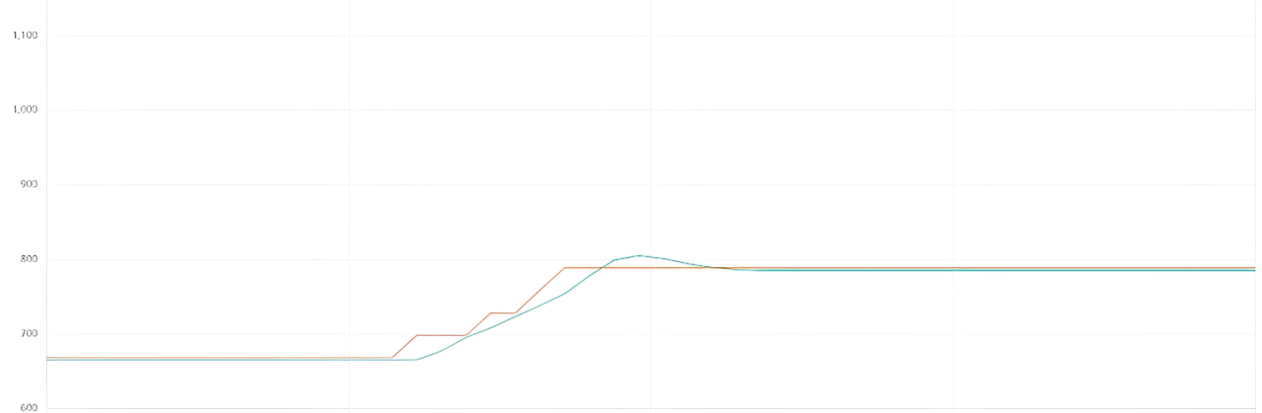
\includegraphics[width=0.9\textwidth]{pd2.png}
	\caption[Hoạt động của hệ thống với bộ điều khiển PD (2)]{Hoạt động của hệ thống với bộ điều khiển PD (2)}
	\label{fig:Hoạt động của hệ thống với bộ điều khiển PD (2)}
\end{figure}

Đổi lại hệ thống hoạt động với độ ổn định cao, không xảy ra hiện tượng dao động.
\newpage
\subsubsection{Với bộ điều khiển PID}

Với bộ điều khiển PID, hệ thống cho thấy độ chính xác cao trong quá trình hoạt động.

 \begin{figure}[h!]
	\centering
	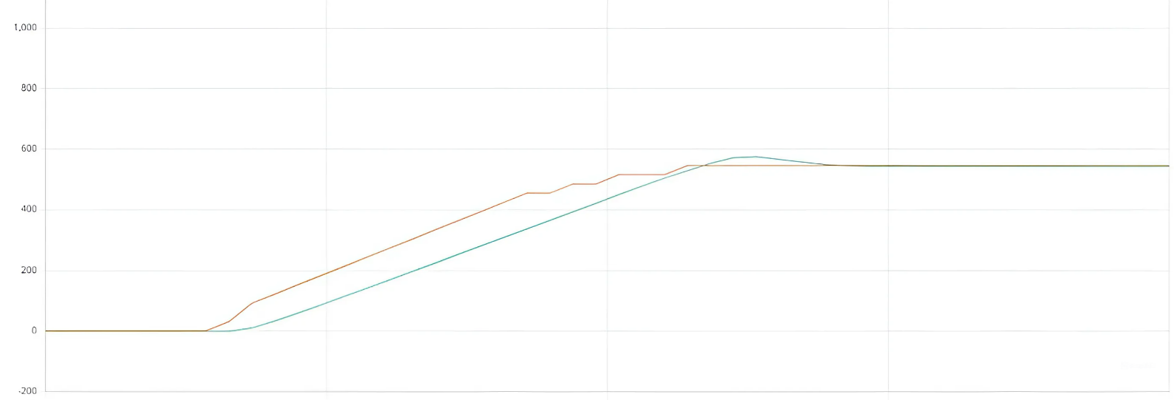
\includegraphics[width=0.9\textwidth]{pid1.png}
	\caption[Hoạt động của hệ thống với bộ điều khiển PID (1)]{Hoạt động của hệ thống với bộ điều khiển PID (1)}
	\label{fig:Hoạt động của hệ thống với bộ điều khiển PID (1)}
\end{figure}

Trong trường hợp giá trị PV chưa bằng SP, thành phần tích phân sẽ tích lũy giá trị sai số và tiếp tục điều khiển động cơ sao cho hai giá trị này bằng nhau. Điều này sẽ giúp cho hệ thống hoạt động với độ chính xác cao.

Tuy vậy, việc tích lũy tích phân sai số cũng sẽ khiến hệ thống mất đi tính ổn định, trong một số trường hợp động cơ còn xảy ra hiện tượng dao động. Nguyên nhân là do ba hằng số độ lợi chưa hoàn toàn tối ưu với hệ thống.

 \begin{figure}[h!]
	\centering
	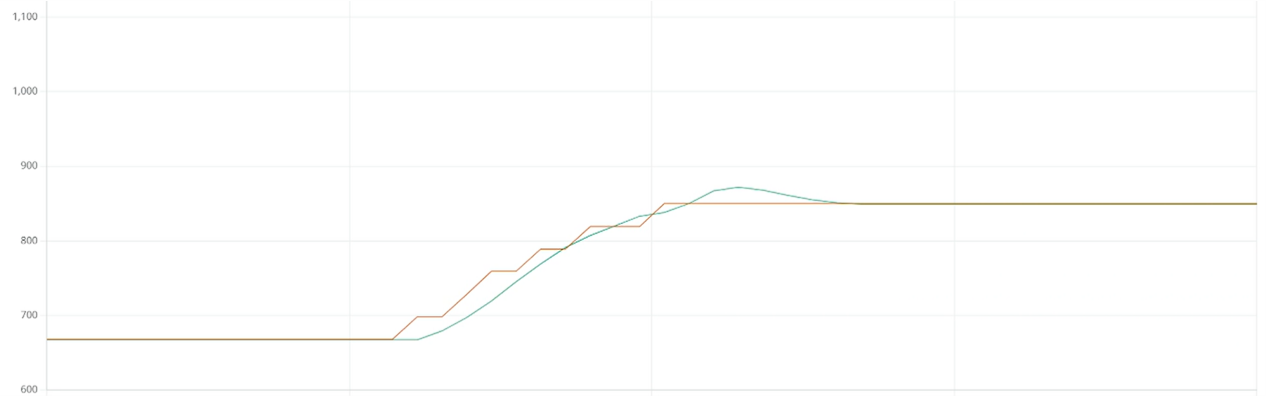
\includegraphics[width=0.9\textwidth]{pid2.png}
	\caption[Hoạt động của hệ thống với bộ điều khiển PID (2)]{Hoạt động của hệ thống với bộ điều khiển PID (2)}
	\label{fig:Hoạt động của hệ thống với bộ điều khiển PID (2)}
\end{figure}
